\documentclass[../sparc.tex]{subfiles}
\graphicspath{{\subfix{../images/}}}
\begin{document}

%%%%%%%%%%%%%%%%%%%%%%%%%%%%%%%%%%%%%%%%%%%%%%%%%%%%%%%%%%%%%%%%%%%%%%%%%%%%%%%%
\section{Аналогово-цифровое преобразование}

Мы могли заметить в главе \ref{section:analog-ports}, что при считывании с
аналогово порта получается значения в диапазоне от 0 до 1023.  Число 1023
подозрительно похоже на число 1024, которое в программировании встречается
достаточно часто -- не удивительно, ведь 1024 это степень двойки ($2^{10}$).

Давайте разберёмся, почему же значения с аналогового порта в Arduino находятся
именно в таком диапазоне.  Начнём с того, что аналоговый порт каким-то образом
преобразует входящий аналоговый сигнал в цифровое (двоичное) представление,
которое мы и видим в программе.

Операцию преобразования аналогового сигнала в цифровой выполняет компонент,
называемый \emph{Аналого-Цифровой Преобразователь} (сокращённо ``АЦП''.)  В роли
АЦП может выступать как отдельная микросхема, так и сам микроконтроллер.
Схематически аналогово-цифровой преобразователь можно изобразить, как показано
на рис. \ref{fig:adc-schematics}.

По-английски ``АЦП'' -- ``Analog-to-Digital Converter'' (сокращённо ``ADC''.)

\begin{figure}[ht]
  \centering
  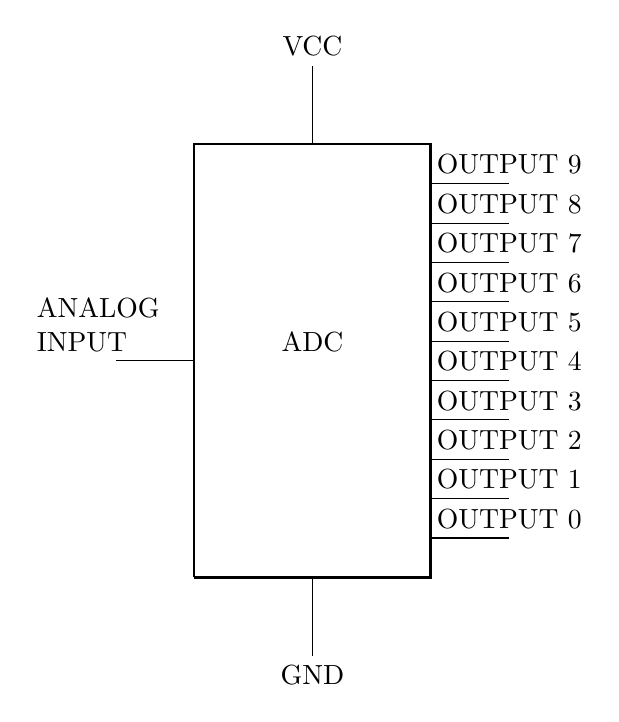
\begin{tikzpicture}
    \draw[thick] (0, 0) -- (0, 5.5) -- (3, 5.5) -- (3, 0) -- (0, 0);
    \draw (1.5, 2.75) node[right, above] {ADC};
    \foreach \n/\y in {0/0.5, 1/1, 2/1.5, 3/2, 4/2.5, 5/3, 6/3.5, 7/4, 8/4.5, 9/5} {
      \draw (3, \y) -- (4, \y) node[right, above] {OUTPUT \n};
    };
    \draw (0, 2.75) -- (-1, 2.75) node[left, above, text width=2cm] {ANALOG INPUT};
    \draw (1.5, 5.5) -- (1.5, 6.5) node[right, above] {VCC};
    \draw (1.5, 0) -- (1.5, -1) node[right, below] {GND};
  \end{tikzpicture}
  \caption{Схематическое изображение аналогово-цифрового преобразователя.}
  \label{fig:adc-schematics}
\end{figure}

На вход АЦП (``ANALOG INPUT'') подаётся аналоговый сигнал, а на выходах
(``OUTPUT 0'' .. ``OUTPUT 9'') кодируется значение входного сигнала в каждый
момент времени в виде набора логических уровней ``HIGH'' (``1'') / ``LOW''
(``0''.)  Самому АЦП требуется также питание -- для этого как раз предназначены
выводы ``VCC'' и ``GND''.

\example { На вход АЦП подаётся 2.5В.  На выходах формируется двоичное значение
  ``1000000000'', что соответствует числу $2^9 = 512$, которое может быть
  получено в программе микроконтроллера. }

Преобразование аналогового сигнала в цифровой внутри АЦП проходит в три этапа:
\begin{enumerate}

\item \textbf{Дискретизация.} Выбираются значения из исходного аналогового сигнала через
  равные временные промежутки (\ref{fig:discretization}.)

  \begin{figure}[h]
    \centering
    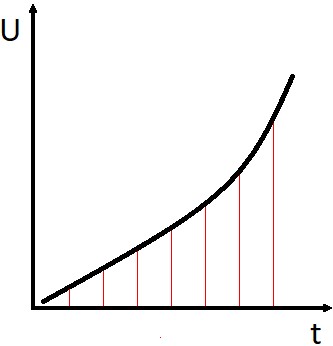
\includegraphics[width=8cm]{discretization}
    \caption{Дискретизация.}
    \label{fig:discretization}
  \end{figure}

  Характеристика, отражающая эти временные промежутки, называется \emph{частотой
  дискретизации}.

\item \textbf{Квантование.} Полученные значения заменяются ближайшим значением из
  набора фиксированных величин -- \emph{уровней квантования}
  (\ref{fig:quantization}.)

  \begin{figure}[h]
    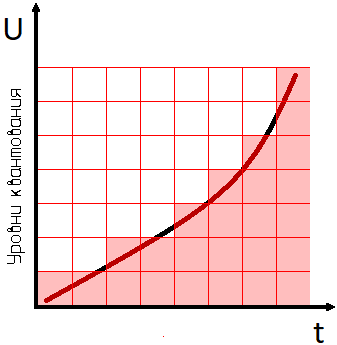
\includegraphics[width=8cm]{quantization}
    \caption{Квантование.}
    \label{fig:quantization}
    \centering
  \end{figure}

\item \textbf{Кодирование.} Квантованным значениям присваивается цифровой код
  (\ref{fig:coding}.)

  \begin{figure}[h]
    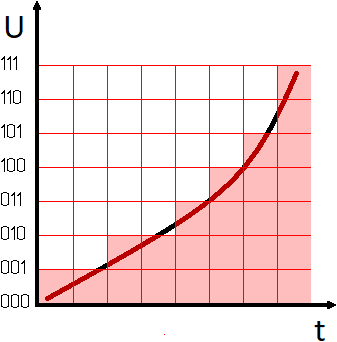
\includegraphics[width=8cm]{coding}
    \caption{Кодирование.}
    \label{fig:coding}
    \centering
  \end{figure}

  Чем выше частота дискретизации и чем больше уровней квантования, тем точнее
  преобразование.

\end{enumerate}

Одной из характеристик АЦП является \emph{разрядность}.  Она определяет диапазон
значений, которое может выдать АЦП.

Компьютеры оперируют двоичной системой исчисления -- то есть, минимальная единица
хранения информации, называемая \emph{бит}, может хранить только одно из двух
значений: один или ноль.

В двух подобных ячейках (битах) мы можем хранить уже 4 комбинации нулей и
единиц: 00, 01, 10, 11.  Если мы возьмём 3 бита, то это даст нам уже 8
комбинаций.  Несложно проследить зависимость: добавление каждого дополнительного
бита увеличивает количество комбинаций в два раза.

Это можно посчитать даже проще: нам не нужно вручную вписывать единицы и нули в
условные ``клетки'' и считать их.  Вместо этого мы можем использовать следующую
формулу:

\begin{equation}
  \mbox{количество комбинаций} = 2^{\mbox{n}}
\end{equation}

Где \texttt{n} -- это количество бит, доступных для хранения значения.

Для примера, если мы возьмём 8 бит для хранения информации, то это даст нам $2^8
= 256$ комбинаций нулей и единиц.

Посмотрим на график (\ref{fig:coding}): для кодирования значений используется
три бита -- значит АЦП, описываемый таким графиком, имеет разрядность 3 бита.  То
есть, количество уровней квантования будет $2^3 = 8$.

Однако нам надо не забывать, что отсчёт в компьютерном мире обычно ведётся с
нуля, и ситуация, когда все биты выставлены в ноль, тоже является одним из
доступных значений диапазона.  Предположим, что нам доступно 8 бит и мы их все
задали, равными единице, то есть $11111111_2$.  Если мы переведём это число в
десятичную форму, то получим:

\begin{equation}
  11111111_2 = (2^7 * 1) + \mbox{...} + (2^2 * 1) + (2^1 * 1) + (2^0 * 1) = 255_{10}
\end{equation}

Таким образом мы видимо, что максимальное положительное значение для 8 бит равно
числу 255.

Из этого оследует, что максимальное значение для \texttt{n} бит можно посчитать
по следующей формуле:

\begin{equation}
  \mbox{количество комбинаций} = 2^{\mbox{n}} - 1
\end{equation}

Из этого следует, что если мы возьмём 10 бит для хранения информации, то в них
мы можем закодировать 1024 комбинаций из нулей и единиц, так как $2^{10} =
1024$.  Но максимальное положительное значение будет равно 1023.  Следовательно
в Arduino АЦП имеет разрядность 10 бит.

Ещё есть такое устройство как ЦАП -- \emph{Цифро-Аналоговый Преобразователь},
который, как нетрудно догадаться, выполняет функцию, обратную функции АЦП -
преобразует цифровой сигнал в аналоговый. Область применения ЦАП и АЦП
достаточно широка: в звуковых и видеокартах, в мониторах, в различной
акустической аппаратуре, в измерительных приборах, и многих других видах
техники.

Стоит упомянуть про 8-битную музыку в древних игровых консолях. Её название
отражает разрядность ЦАП звуковых чипов тех консолей -- 8 бит. Именно такой ЦАП
позволял выдавать тот самый резковатый, хлопающий и шипящий звук.

\end{document}
